\documentclass{ecnreport}

\stud{Control \& Robotics master}
\topic{C++ Programming}

\begin{document}

\inserttitle{C++ Programming exam}
\insertsubtitle{Group 1}

\section{Context}

Sudoku is a popular game that is played on a $9\times$ 9 grid, some cells containing digits between 1 and 9 and some empty.
Playing the game amounts to filling the grid with only 4 rules:
\begin{itemize}
 \item Each cell should have a digit between 1 and 9
 \item Each row should contain all digits
 \item Each column should contain all digits
 \item Each of the 9 sub-square of dimension $3\times 3$ should contain all digits
\end{itemize}

The difficulty of a Sudoku represents how many candidates exist in each empty cell at the beginning. An easy Sudoku will contain some cells having only one candidate, leading to a sure guess. A difficult Sudoku will contain only cells having several candidates, forcing the player to rely on hypotheses until a contradiction occurs.


\begin{figure}[h!]\centering
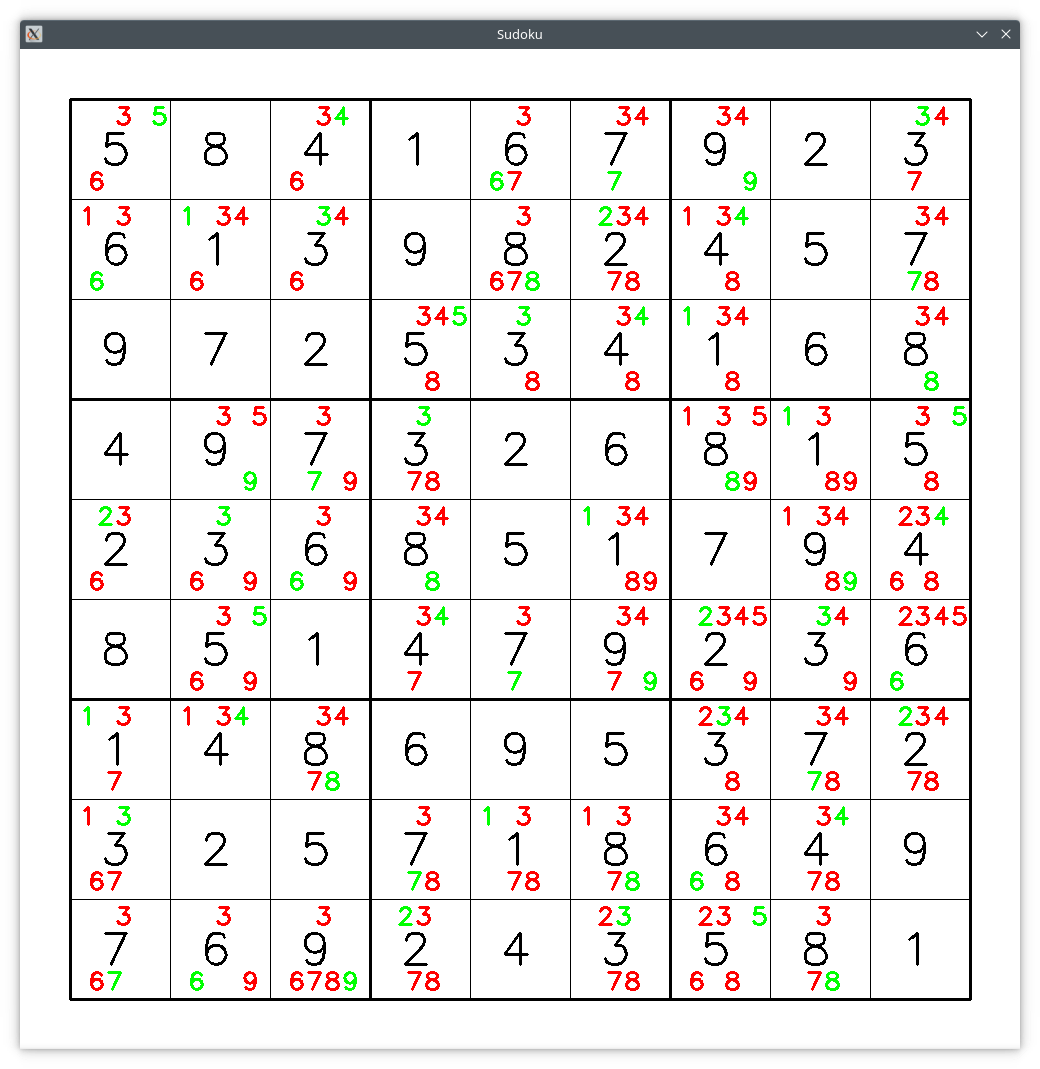
\includegraphics[width=.5\linewidth]{sudoku.png}
\caption{A solved Sudoku. Red digits show initial candidates for each cell. Green digits are the initial candidate that was the valid one at the end. Cells without red/green digits are the ones from the starting grid.}
\label{fig:trilat}
\end{figure}

\section{Backtracking algorithm}

Backtracking is a simple algorithm that can solve Sudoku quite well. It solves the cells one at the time, possibly doing a guess among the candidate digits. If it finds a contradiction, is cancels the previous guess and tries the next one. For an easy Sudoku, this algorithm will never have to do any wild guess and will solve the grid without ever cancelling a guess.\\
\newcommand{\var}[1]{\texttt{\upshape #1}}

The algorithm reads as follows, under the \var{solveNextCell()} function.\\
This function is recursive as once a guess is done on a cell, it calls \var{solveNextCell()} again.

 \begin{algorithm}[!h]
 \DontPrintSemicolon
 \SetKwFunction{Fill}{{\bf Function} solveNextCell}\;
 \Fill{}
 {
 \\
 \If{\var{grid} is full}{\Return \var{true}\;}
\var{next\_cell} $\gets$ best next cell to investigate\;
\For{\var{guess} in \var{next\_cell.candidates}}{
\If{\var{next\_cell} could be \var{guess}}
{
 \tcp{the guess is compatible with the cell's neighboors}
Assign \var{guess} to \var{next\_cell} \tcp{also prune from \var{neighboors}}
\If{\var{solveNextCell()}}{\Return \var{true}\; }
\tcp{\var{guess} leads to some contradiction}
Cancel \var{guess} for \var{next\_cell} \tcp{also restore it from \var{neighboors}}
}
}
\tcp{We have tried all candidates for this cell, without success}
\Return \var{false}\;
}
% \SetAlgoLined

\caption{Backtracking algorithm}
\label{backtracking}
\end{algorithm}

As we can see the algorithm relies on a few underlying functions, that are expressed as methods (member functions) of the \texttt{Cell} class:

\begin{itemize}
 \item A \texttt{Cell} should be able to tell if a given guess could be set as its digit
 \item A \texttt{Cell} should be able to set a guess and prune it from its neighboors
 \item A \texttt{Cell} should be able to cancel a guess and restore it for its neighboors
\end{itemize}

Additionally, a grid should be able to tell if it is full, that is all its cells have a digit.

\newpage
\section{Available classes and methods to implement}

\def\Grid{\texttt{Grid}~}
\def\Cell{\texttt{Cell}~}

The \texttt{main} function is quite trivial and only loads the desired Sudoku to solve. The algorithm itself is done through two classes: \Grid and \Cell.

\subsection{\Grid class}

The \Grid class has:
\begin{itemize}
 \item An array of 81 \Cell called \texttt{cells}
 \item A \texttt{solve()} method that enters the solving process and prints the outcome
 \item A \texttt{solveNextCell()} method that implements the backtracking algorithm
\end{itemize}

\fbox{You have to implement the \texttt{solveNextCell()} method as shown in Algorithm \ref{backtracking}.}

\subsection{\Cell class}

As seen above, most of the intelligence comes from the cell being able to change its guess and inform its neighboors.
The \Cell class has:
\begin{itemize}
 \item A \texttt{unsigned int} called \texttt{digit} that is the current guess for this cell. If \texttt{digit} is 0 it means this cell was not assigned a value at this point of the algorithm
 \item A vector of \texttt{unsigned int} called \texttt{candidates} that lists the remaining candidates at any point during the algorithm
 \item An array of \texttt{unsigned int} called \texttt{pruned} that tells how many times a given digit was pruned for this cell. Index 0 is not used so for example \texttt{pruned[3]} tells how many times 3 was said to be a forbidden value for this cell. When \texttt{pruned[3]} balls back to 0, 3 should be added to the \texttt{candidates} again
 \item An array of 20 pointers to \Cell called \texttt{neighboors} that point to all other cells that cannot have the same digit as this one
 \item Many member functions to deal with bookkeeping of pruned values and candidates
 \item Two static functions \texttt{isAssigned(cell)} and \texttt{isValid(cell)} to be used in algorithms
 \item 4 member functions that are called by the backtracking algorithm: \texttt{couldBe(guess)}, \texttt{canPrune(guess)}, \texttt{setGuess(guess)} and \texttt{cancelGuess(guess)}
\end{itemize}

\fbox{You have to implement these four last methods, their definition being listed below}

\paragraph{\bf \texttt{bool couldBe(unsigned int guess)}}~\\

 \begin{minipage}{.5cm}
~
 \end{minipage}
 \begin{minipage}{0.9\linewidth}
    This method should return \texttt{True} if the cell could have the requested value.\\
    Two conditions should be met:

\begin{itemize}
 \item The cell does not have a digit yet, or its digit is equal to the guess
 \item {\bf and} the requested guess can be pruned from all its neighboors
\end{itemize}
 \end{minipage}




\paragraph{\texttt{bool canPrune(unsigned int guess)}}~\\

 \begin{minipage}{.5cm}
~
 \end{minipage}
 \begin{minipage}{0.9\linewidth}
This method should return \texttt{True} if the cell could be different from the requested value. Several conditions should be combined:
\begin{itemize}
 \item If the cell has a valid digit already, returns whether this digit is different from the guess
 \item \texttt{False} if the cell has not a valid digit yet but has only one remaining candidate, that is equal to the guess. In this case, pruning this guess would make the cell without digit and with no remaining candidate.
 \item \texttt{True} otherwise: the cell has several candidates so it can be pruned from one.
\end{itemize}
 \end{minipage}


 \paragraph{\texttt{bool setGuess(unsigned int guess)}}~\\

 \begin{minipage}{.5cm}
~
 \end{minipage}
 \begin{minipage}{0.9\linewidth}
This method should set the guess on this cell and prune it from its neighboors
% \begin{itemize}
%  \item Set digit to the guess
%  \item Call the \texttt{prune} method on all its neighboors
% \end{itemize}
 \end{minipage}

  \paragraph{\texttt{bool cancelGuess(unsigned int guess)}}~\\

 \begin{minipage}{.5cm}
~
 \end{minipage}
 \begin{minipage}{0.9\linewidth}
This method should cancel the guess on this cell and restore it from its neighboors
% \begin{itemize}
%  \item Set digit to 0
%  \item Call the \texttt{restore} method on all its neighboors
% \end{itemize}
 \end{minipage}

 \subsection{Tips}

 All the methods can be written in a few lines by using modern C++ that is:
 \begin{itemize}
  \item range-based for loops
  \item \texttt{<algorithm>} functions such as \texttt{std::any\_of} and \texttt{std::all\_of}, possibly with lambda or existing functions
 \end{itemize}

 Some basic errors will lead to the program crashing, {\bf use the debugger} to understand what went wrong.
\\
You can also use it with breakpoints to see what is going on in this mess.\\

Do not modify parts of the code you are not supposed to implement or you will never be able to solve a Sudoku again.


\newpage


\subsection{Bonus: improve the \texttt{bestNextCell} function}

In \texttt{grid.cpp} the \texttt{bestNextCell} function takes two \Cell called \texttt{c1, c2} and returns whether \texttt{c1} should be investigated before \texttt{c2}. The initial function just compares the cells' digit, ensuring that a cell with digit 0 (e.g. no guess yet) will always be chosen over a cell that is already set.

This may lead the algorithm to start with cells that have a large number of candidates, while some others may have less and even only one. Improve this function as you think is best and compare the solving times.

\subsection{Bonus: keep track of the algorithm back and forth}

The \Grid class has member variables called \texttt{guesses} and \texttt{cancels} that are printed at the end. Update them in the \texttt{solveNextCell} function to see what happens under the hood.

\subsection{Huge bonus: find my bug}

When trying to do smarter things in the \texttt{bestNextCell} function the solver sometimes (e.g. depending on the initial grid) tells that there is no solution to the grid. I have no idea why.


\section{Starting grids}

The \texttt{starts} folder lists several starting grids, to be set in the \texttt{main} function to test your algorithm:
\begin{itemize}
 \item \texttt{basic0} is already filled. You should start with that to test the exit criterion.
 \item \texttt{basic1} and \texttt{basic2} have respectively only 1 and 2 empty cells
 \item \texttt{easy}, \texttt{medium}, \texttt{hard} and \texttt{harder} are of increasing complexity
\end{itemize}



\end{document}
